\documentclass[final,1p,12pt]{elsarticle}

%% The amssymb package provides various useful mathematical symbols
\usepackage{amssymb}
%% The amsthm package provides extended theorem environments
\usepackage{amsthm}
%% The amsmath package provides binomial notation for us
\usepackage{amsmath}
%% The parcolumns package provides multiple columns for examples.
\usepackage{parcolumns}
% The tikz package provides drawings for Combinations set notation (Venn Diagram).
\usepackage{tikz}
%% Removes the wonky "Preprint Submitted to Elsevier" and adds a front-page footer. 
\makeatletter
\def\ps@pprintTitle{%
 \let\@oddhead\@empty
 \let\@evenhead\@empty
 \def\@oddfoot{
    \hspace*{\fill}
    {Compiled by John Oss} \hfill {\thepage} \hfill{\@journal\today}
    \hspace*{\fill}}%
 \let\@evenfoot\@oddfoot}
\makeatother

%% Definitions
\newtheorem{definition}{Definition}
\newtheorem{example}{Example}

%% Start of Document
\begin{document}

%% Header
\begin{frontmatter}
    \title{Exam Notes for MDM4UI}
        \begin{abstract}
        Notes for all topics taught in MDM4UI (Data Management) from the winter term of the 2016-2017 school year at GCI.  Please refer to Appendix A for a walkthrough of example questions that will probably be on the exam. Sorry for the formatting. I'm not quite done yet.
    \end{abstract}
\end{frontmatter}

%% Body 
\section{Permutations}
Permutations are the arrangements of objects in a set order. 
For instance, how many ways can you rearrange the letters in the word "APPLE", 
or how many ways can you bring 4 people out of 20 friends to a party.

    \subsection{Factorial Notation}
    Often in permutations, we need to multiply descending consecutive numbers. Since these numbers
    are descending and not ascending, we can safely assume that \textbf{every factorial must be positive}. 
    For instance,  $5\times4\times3\times2\times1$ can often be simplified and written as \textbf{5!}, or 5 factorial.\\
    The general rule for factorial notation is: 
    \begin{equation}%Factorial Equation
        n! = n\times(n-1)\times(n-2)\cdots3\times2\times1
    \end{equation}
    The exception to this rule is 0!, which in this case would be $0! = 1$, which would follow the same thinking as $n^0=0$.%%Complete
    
    \subsection{Rule of Product and Rule of Sum}
    How many different results can one get from flipping a coin 3 times? You have 2 possibilities, heads or tails, and you flip it 3 times. Essentially, you have three groups of two, or $2\times3$ different results, which turns out to be $6$ different possible results. This is called the \emph{Fundamental Rule of Product} or the \emph{Counting Principle}
    \begin{definition}
        The Rule of Product states that if the 1st action can be performed in n ways, and the 2nd action can be performed in m ways.
        They can be performed together in $n\times m$ ways. 
    \end{definition}
    \clearpage
    What happens if the actions cannot be performed together? Such as which car to buy? In that case we have another rule, known as the \emph{Rule of Sum}.
    \begin{definition}
        The Rule of Sum states that if the 1st action can be performed in n ways, and the 2nd action can be performed in m ways, and these actions cannot occur together, then there are $n+m$ ways for either of the actions to occur.
    \end{definition}
    
    \subsection{N-Arrangements}
    Let's say you have 5 people, and you need to arrange them in a line.
    You put one person in the first spot, and now you have 4 left. Repeat this until you are left with one person, which fits into the last spot. You can express this mathematically by writing out $5\times4\times3\times2\times1$ or $5$ factorial.\\
    This is quite similar to the Rule of Product as:
    \begin{enumerate}
        \item Each placement is a choice
        \item The number of choices is reduced with each previous action. 
    \end{enumerate}
    A permutation of \emph{n} objects is an arrangement of the objects in a \textbf{definite order}. This can be expressed with permutation notation, shown below where P(n,n) equals the number of ways to permute n objects.
    \begin{equation}
        P(n,n) = n!
    \end{equation}
    This equation will only work when the number of spaces to occupy and the number of objects are equal. In other cases we'll have to use an r-arrangement.
    
    \subsection{R-Arrangements}
    If you have more objects than places you can put the objects into, then we can use something called an r-arrangement. An r-arrangement is a permutation of \emph{n} objects taken \emph{r} at a time, as is shown below.
    \begin{equation}
       P(n,r) = \frac{n!}{(n-r)!} 
    \end{equation}
    Where $P(n,r)$ equals the total number of arrangements you have, divided by the number of unused objects. This is most commonly displayed on calculators as \emph{nPr}. For example you have 4 subjects, but you can only study two at a time. The equation for that would be $\frac{4!}{(4-2)!}=12\mbox{ combinations.}$ 
\clearpage
    
    \subsection{Permutations with Repeating Elements}
    All previous examples will ONLY work with non-repeating elements, such as the letters in the word "MONTREAL", or 5 different books. They will definitely NOT work for questions with repeating elements, such as the word "FIJI". For all repeating elements we'll have to follow another rule shown below.
    \begin{definition}
        In general, the number of arrangements of \emph{n} objects of which \emph{a} of one kind are alike, and \emph{b} of one kind are alike and so forth is given by the expression below, Where the number of permutations can be found by dividing the total number of possible combinations by the repeating elements.
        \begin{equation}
            \frac{n!}{a!b!c!\cdots}
        \end{equation}
    \end{definition}
    
    \subsection{Problem Solving with Permutations}
    There are 3 methods for solving problems with permutations. They are called: the Indirect Method, the Case Method, and Circular Arrangements.
    
        \subsubsection{Indirect Method}
        The indirect method involves taking all possibilities and subtracting those which are not wanted. For instance, say you have 3 people that need to sit at a table, but 2 of them don't want to sit beside each other. There is a step-by-step process that you can use for this question that is explained below.
        \begin{enumerate}
                \item Find all possible permutations (ex. P(3,3) )
                \item Find all unwanted permutations (in this case when they are together)
                \item Subtract the unwanted permutations from the wanted permutations.
            \end{enumerate}
        This can be written as:
        \begin{equation}
            \mbox{\textbf{Wanted Outcomes}} = \mbox{Total Outcomes}-\mbox{Unwanted Outcomes}
        \end{equation}
    
        \subsubsection{Case Method}
        The Case Method involves breaking down the equation into manageable parts, then adding them to get the final solution. There is a step-by-step example problem in Section 1 of the appendix, along with an explanation of why, and how you manage the "breaking into parts" aspect.

    \clearpage
    
        \subsubsection{Circular Arrangements}
        Circular arrangements are no longer a part of the curriculum, and as such they will not be tested on, but they are still quite useful to know in niche cases. If you have seven people seated at a table, and they all move to their rights, their positions may have moved, but their order remains the same, think of it like a circle. Keep in mind that if there is some fixed point, the question just ends into a typical linear arrangement, with the equation simplifying to $1 \times (n-1)!$.
        
\section{Combinations}
A Combination is a way of selecting objects (permuting) from a group, without the order being important. In essence, it is orderless permutations. Let $ABC$ be a permutation. In Section 1, we asserted that $ABC$ and $BAC$ are different, as their orders are different. In combinations, we assert that $ABC$ and $BAC$ are the same, as they contain the same objects, just in a different order.

    \subsection{Set Theory}
    Set Theory involves the creation and manipulation of sets and their properties. A set is a collection of distinct objects in which their order does not matter. The objects in this set are called elements. If a set does not have any elements in it, we refer to it as a \emph{null set}, which is shown as $\emptyset$ or $(\emptyset)$. This null set is a subset of everything. If we want to describe a set containing elements, we must follow the example below.
    \begin{equation}
        X = \{a,b,c,d,e,f,\cdots,y,z\}
    \end{equation}
    If we wish to describe the number of elements in the set, we can use $n(X)$, where X represents the set, and n returns the number of elements in that set. In this case $n(X) = 26$, as set X contains all the letters of the alphabet. Sets are referred to differently when compared to other sets, as defined below.
    \begin{definition}
    Special Properties of Sets when Compared to Other Sets
    \begin{enumerate}
        \item If two sets have no elements in common they are called disjoint sets.
        \item If two sets have all elements in common they are equal.
        \item If all of elements of A are also in B then A is a subset of B $(A\subseteq B)$
    \end{enumerate}
    \end{definition}
    
        \subsubsection{Universal Set and Complement Sets}
        The set of all elements being considered is called the\emph{universal set} and is always denoted by $S$. When referring to a set of all elements that are in the universal set, but\textbf{ not in set A}, we call this the complement of $A$ or $A`$. For example:
        \begin{equation}
            S = \{1,2,3,4\}, A = \{1,3\}, A`=\{2,4\}
        \end{equation}
        
        \subsubsection{Unions and Intersections}
        For two sets of A and B, the \textbf{union} of A and B or $A\cup B$, is the set of all elements in A or B, not including duplicates.
        \begin{equation}
            S = \{1,2,3,4\}, A = \{1,3\}, B =\{1,2\}, A\cup B=\{1,2,3\}
        \end{equation}
        For two sets of A and B the \textbf{intersection} of A and B, $A\cap B$, is the set of all the elements that are in both set A and set B.
        \begin{equation}
            S = \{1,2,3,4\}, A = \{1,3\}, B =\{1,2\}, A\cap B=\{1\}
        \end{equation}
        If you are ever having trouble remembering the difference between the symbols representing the union and the intersection, remember that a union looks like a cup, and intersection looks like a cap.
        
        \subsubsection{Subsets}
        Subsets, are sets that are also in another set. To find every possible subset (including null set) we need to use the equation:
        \begin{equation}
            2^{n(X)}
        \end{equation}
        In this case, n(X) is the number of elements in Set X. If a question comes up, where we need the number of subsets of a given set with the length $y$, of set $x$, we'd simply use $\binom{n(x)}{y}$
        
    \subsection{Introduction to Combinations}
    A combination is a selection of r objects, from n distinct objects \emph{without regard for order}. The equation for solving combinations is written below.
    \begin{equation}
        C(n,r) = \frac{n!}{(n-r)!\times r!}
    \end{equation}
    This equations finds all combinations by dividing number of objects, by the unused objects $(n-r)!$ and the order of the selected objects. This can be further simplified to:
    \begin{equation}
        C(n,r) = \frac{P(n,r)}{r!}
    \end{equation}
    If order does not matter, the process is called a \emph{Combination}, whereas when order does matter, it is called a \emph{Permutation}. On your calculator, the formulae for combinations will be shown as \textbf{nCr}. If written out by hand, we will use the form:
    \begin{equation}
        \binom{n}{r} = \frac{n!}{(n-r)!\times n!}
    \end{equation}
    Or simply \(\binom{n}{r}\).
    
    \subsection{Inclusion\textemdash Exclusion Principle}
    The Inclusion-exclusion principle is a method of obtaining the number of elements in finite sets. Typically used when asked for the number of combinations of two things, where there is overlap between the two.\\
    Let A represent Set A, and let B represent Set B.
    \begin{center}
        %% Thank you http://tex.stackexchange.com/questions/9681/how-to-draw-venn-diagrams-especially-complements-in-latex
        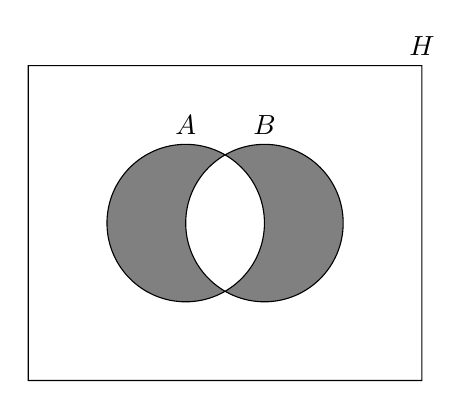
\begin{tikzpicture}[fill=gray]
            % left hand
            \scope
            \clip (-2,-2) rectangle (2,2)
                  (1,0) circle (1);
            \fill (0,0) circle (1);
            \endscope
            % right hand
            \scope
            \clip (-2,-2) rectangle (2,2)
                  (0,0) circle (1);
            \fill (1,0) circle (1);
            \endscope
            % outline
            \draw (0,0) circle (1) (0,1)  node [text=black,above] {$A$}
                  (1,0) circle (1) (1,1)  node [text=black,above] {$B$}
                  (-2,-2) rectangle (3,2) node [text=black,above] {$H$};
        \end{tikzpicture}
    \end{center}
    This diagram perfectly represents the overlap between the two sets. If you caught it earlier, what we're actually finding is $A\cup B$. The Inclusion\textemdash Exclusion Principle is merely a way of finding it algebraically. This image represents the equation below.
    \begin{equation}
        |A\cup B| = |A| + |B| - |A\cap B|
    \end{equation}
    
\section{Independent Study Units}

    \subsection{Modelling with Matrices (ISU 1)}
    
        \subsubsection{Intro to Matrices}
        A matrix is a rectangular array of numbers that is used to organize data. If you are used to computer programming, you will recognize them as 2D arrays. If you are good with set notation, they are in essence, a set of sets. Matrices follow the format below:
        \begin{equation}
            X =
            \begin{bmatrix}
                a & b & c \\
                d & e & f
            \end{bmatrix}
        \end{equation}
        Matrices have various properties, and unique terms created to describe them. For instance, looking at the matrix above, we can safely say that $a$ in an entry, as defined below.
        \begin{definition}Entry:
            An entry refers to a number in a matrix.
        \end{definition}
        How did we figure out the number of entries in the matrix? Simple, we can use the matrix's \emph{dimensions} to figure that out.
        \begin{definition}Dimensions:
            These refer to the size of the matrix, described by the number of rows and columns. The formula below is used to solve for dimensions, where D is the result, $R$ is the rows, and $C$ is the columns.
            \begin{equation}
                D = R \times C
            \end{equation}
        \end{definition}
        
        \subsubsection{Variations and Classifications of Matrices}
        Matrices can be transformed, and compared to each other, much like sets. The definitions of the variations and classifications of the matrices are listed below.
        
        \begin{definition}Transpose Matrix: 
            A transpose matrix is a matrix obtained by interchanging the rows and columns. This is written as $X^{+}$. Shown below is Matrix W, and the transposed equivalent.
            \begin{equation}
                W =
                \begin{bmatrix}
                    a & b & c \\
                    d & e & f
                \end{bmatrix}
                -> X^{+} =
                \begin{bmatrix}
                    a & d \\
                    b & e \\
                    c & f
                \end{bmatrix}
            \end{equation}
        \end{definition}
        
        \begin{definition}Column Matrix:
        A Column Matrix is a matrix that has only one x value. Instead of rows and columns, it is merely a column. For instance, Matrix X in this case would be a Column Matrix.
        \begin{equation}%Column Matrix
            X =
            \begin{bmatrix}
                a&\\
                b&\\
                c
            \end{bmatrix}
        \end{equation}
        \end{definition}
        
        \begin{definition}Row Matrix:
        A Row Matrix is a matrix that has only one y value. It is the transpose of the Column Matrix For instance, Matrix Y in this case would be a Row Matrix.
        \begin{equation}%Row Matrix
            Y =
            \begin{bmatrix}
                a & b & c
            \end{bmatrix}
        \end{equation}
        \end{definition}
        
        \begin{definition}Square Matrix:
        A Square Matrix is a matrix in which the rows and columns are equal. For instance, Matrix Z below is a Square Matrix.
        \begin{equation}%Column Matrix
            Z =
            \begin{bmatrix}
                a&b&c\\
                d&e&f\\
                g&h&i
            \end{bmatrix}
        \end{equation}
        \end{definition}
        
%% Appendix, containing extra practice questions, typically discussed in class, or questions that have been on tests as bonus, or other assorted challenging questions. 

        \subsubsection{Operations with Matrices}
        

\clearpage\appendix
\section{Example Equations Explained}

    \subsection{Permutations}
        \subsubsection{Factorial Notation}
            \begin{example}
            Solve the following equation for n. State restrictions.
            \[\frac{n!}{(n-3)!}=2n\]
            \end{example}
            To solve for n, we must first divide out the denominator, which in this case is $(n-3)!$. Before all of this, we should state our restriction. Since a factorial may not be negative, and $(n-3)!$ would equal $-3!$ our restriction is that \emph{$n\geqslant3$}. You may notice there is no $(n-3)!$ in the top, but the solution for this is simple. If you recall the equation for factorial notation, we can expand the top of this question.  Following this, the equation expands to:
            \[\frac{n\times(n-1)\times(n-2)\times(n-3)!}{(n-3)!}=2n\]
            Next, the $(n-3)!$s cancel out, to bring you this:
            \[n\times(n-1)\times(n-2) = 2n\]
            Now we can divide out the n from both sides. To get this:
            \[(n-1)\times(n-2) = 2\]
            We can't divide any further, so we'll need to expand.
            \[n^2 -3n+2 = 2\]
            Move the 2 over so we can turn this into something we can factor.
            \[n^2 -3n=0\]
            Use factor by grouping to factor this equation.
            \[n(n-3)=0\]
            So either $n=0$ or $n-3=0$. Following our restriction, n be greater than 3, so $n=0$ is inadmissible, so our answer must be $n=3$.
    \clearpage
        \subsubsection{Rule of Product and Rule of Sum}
            \begin{example}
            Using only the numbers from $0\cdots4$, how many three digit numbers can you find if the number $4$ \textbf{MUST} be included. No repetition.
            \end{example}
            For this question we must follow the Rule of Sum.
            
    \clearpage
        \subsubsection{Problem Solving with Permutations}
            \begin{example}
            Try to find the total number of arrangements of the numbers 0-7(8 digits) that are even. No repetition is allowed, and the number cannot start with a 0.
            \end{example}
            For this question, you can use the \textbf{Case Method} and break the question down into numbers that end in a zero, and numbers that don't end in a zero, yet still end in an even number. 
            \begin{parcolumns}{2}
                \colchunk[1]{\\\textbf{Numbers that end in a zero:}
                    $$7! \times 1 = 5040$$
                    \\\textbf{Explanation:} One has 7 possible numbers for the first place, and only zero as the final possible number.
            }
                \colchunk[2]{\\\textbf{Numbers that end in 2,4,6:}
                    $$6 \times 6 \times 3 = 12960$$
                    \\\textbf{Explanation:} The last number is 3, and represents the possible even numbered endings (2,4,6). The reason why it is $6 \times 6$, it is because zero cannot be first, yet it can be second\\
            }
            \colplacechunks
            \end{parcolumns}
            This question isn't over yet though. Finally, you will have to add the solutions together, as you may have found all of the answers for the possible even numbers (0,2,4,6), but they haven't been added together yet.
            $$5040 + 12960 = 18000$$
            \emph{In conclusion}, there will be 18000 possible combinations of even numbers by using the numbers 0-7 (8 digits in total).
            
    \subsection{Combinations}
        \subsubsection{Set Theory}
    \clearpage
        \subsubsection{Intro to Combinations}
            
            \begin{example}
                A committee of 4 people is chosen from 10 students, 6 parents, and 10 teachers. Order does not matter. How many ways can we make the committee if there are a) no restrictions and b) At least one teacher.
            \end{example}
                \textbf{a) No restrictions:}
                 We can assume that this is a combination, as there are no restrictions other than order does not matter. Therefore we only need to fill in the combination equation, which turns out to be C(26,4). 
                 $$\binom{26}{4} = 14,950$$
                 \textbf{b) At least one teacher.}
                 There are two ways to handle this question, we can solve it either directly, or indirectly. In this example, I will choose indirectly. In this case, we want every solution with a teacher in it, and do not want the solution with zero teachers. Therefore we must subtract the unwanted solutions from all the solutions. This would work out to be:
                 $$\binom{26}{4} - \binom{10}{0}\times\binom{16}{4} = 13130$$
        

%% References
%%
%% Following citation commands can be used in the body text:
%% Usage of \cite is as follows:
%%   \cite{key}         ==>>  [#]
%%   \cite[chap. 2]{key} ==>> [#, chap. 2]
%%

%% Possible sections:
%% \section{Practice Questions}
%% \section{Practice Answers}

    \subsection{Google Sheets (ISU 2)}
    
\end{document}

%%
%% EOF